\chapter{\MakeUppercase{Methodology and Testing}}

\section{Methodology Overview}
\paragraph{}

For this project, I followed an experiment-based methodology to study one main question: if we increase fairness constraints in credit scoring, how much model performance changes.

Instead of testing only one model or one fairness setting, I compared multiple models and multiple fairness levels under the same data pipeline. This helped keep the comparison fair and meaningful.

\section{Experimental Setup}
\paragraph{}

The experiments were run by varying three things:
\begin{itemize}
    \item Dataset
    \item Model
    \item Fairness level
\end{itemize}

For each combination, I used the same preprocessing and evaluation method so results are comparable.

The fairness levels used were:
\begin{itemize}
    \item 0.0 (baseline, no fairness constraint)
    \item 0.25
    \item 0.5
    \item 0.75
    \item 1.0 (strongest fairness constraint)
\end{itemize}

\section{Data Methodology}
\paragraph{}

The project works on public credit datasets configured in the pipeline.

Each dataset has:
\begin{itemize}
    \item A target variable (loan/credit outcome)
    \item A protected attribute (used for fairness analysis)
\end{itemize}

Data preparation includes:
\begin{itemize}
    \item Handling missing values
    \item Encoding categorical columns
    \item Scaling numeric columns
\end{itemize}

To evaluate models properly:
\begin{itemize}
    \item Data is split into train/test (80:20, stratified)
    \item 5-fold stratified cross-validation is used on training data
\end{itemize}

A fixed random seed (42) is used to make runs reproducible.

\section{Model Methodology}
\paragraph{}

I evaluated six models:
\begin{itemize}
    \item Logistic Regression
    \item Decision Tree
    \item Random Forest
    \item Gradient Boosting
    \item Explainable Boosting Machine (EBM)
    \item XGBoost
\end{itemize}

For each model, I ran:
\begin{itemize}
    \item Baseline training (no fairness constraint)
    \item Fairness-constrained runs at higher fairness levels
\end{itemize}

This way, each model can be checked for both predictive power and fairness behavior.

\section{Fairness Methodology}
\paragraph{}

Fairness constraints were applied using Fairlearn’s constrained optimization approach (Exponentiated Gradient). The idea is to gradually increase fairness pressure and observe what changes in model outcomes.

Fairness was measured using:
\begin{itemize}
    \item Demographic Parity Difference
    \item Equalized Odds Difference
    \item Disparate Impact Ratio
\end{itemize}

I also tracked subgroup gaps (selection rate and TPR gaps) to understand group-level behavior better.

\begin{figure}[h!]
    \centering
    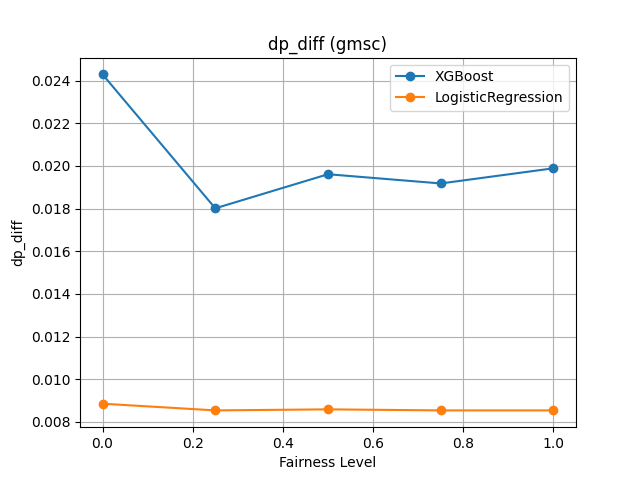
\includegraphics[width=0.8\textwidth]{images/gmsc_dp_diff.png}
    \caption{Demographic Parity Difference vs Fairness Level (GMSC)}
\end{figure}

\begin{figure}[h!]
    \centering
    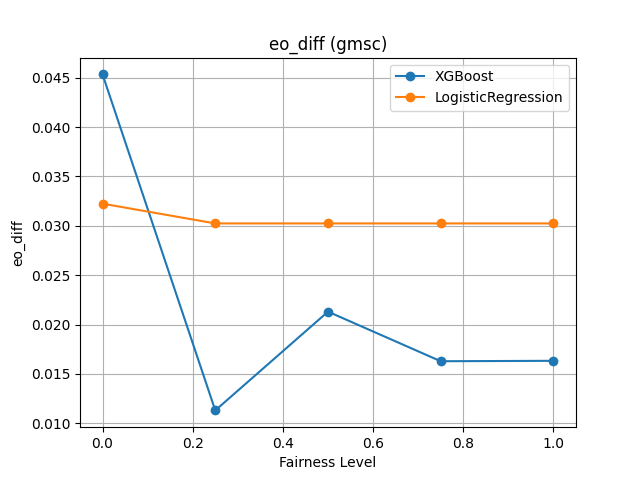
\includegraphics[width=0.8\textwidth]{images/gmsc_eo_diff.png}
    \caption{Equalized Odds Difference vs Fairness Level (GMSC)}
\end{figure}

\begin{figure}[h!]
    \centering
    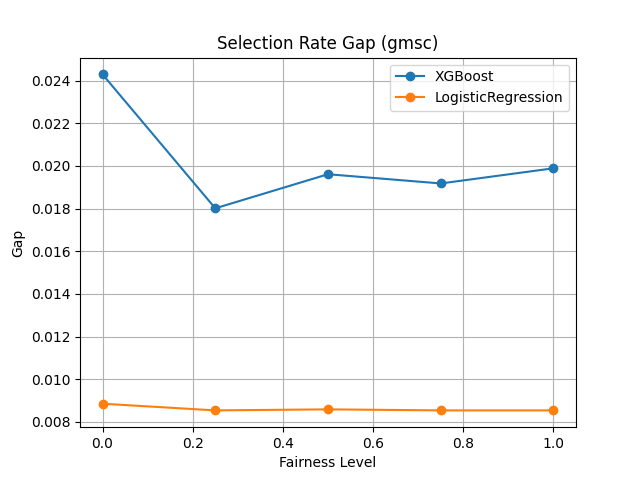
\includegraphics[width=0.8\textwidth]{images/gmsc_selection_gap.png}
    \caption{Selection Rate Gap Across Fairness Levels (GMSC)}
\end{figure}

\begin{figure}[h!]
    \centering
    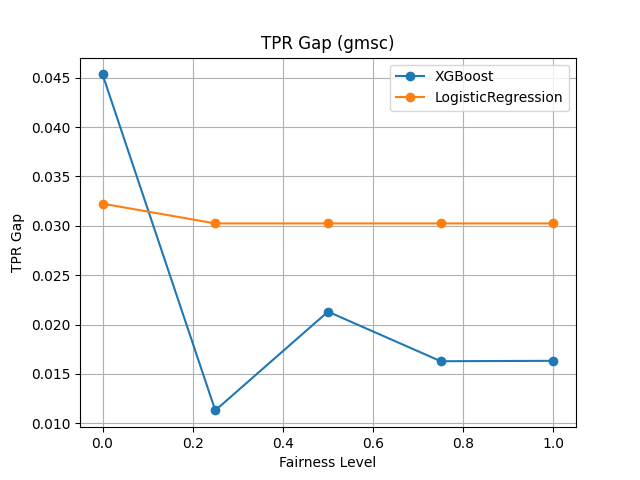
\includegraphics[width=0.8\textwidth]{images/gmsc_tpr_gap.png}
    \caption{TPR Gap Across Fairness Levels (GMSC)}
\end{figure}

\section{Performance Evaluation Metrics}
\paragraph{}

Model performance was measured using:
\begin{itemize}
    \item Accuracy
    \item ROC-AUC
    \item F1 Score
\end{itemize}

These three metrics together give a more balanced view than accuracy alone.

\begin{figure}[h!]
    \centering
    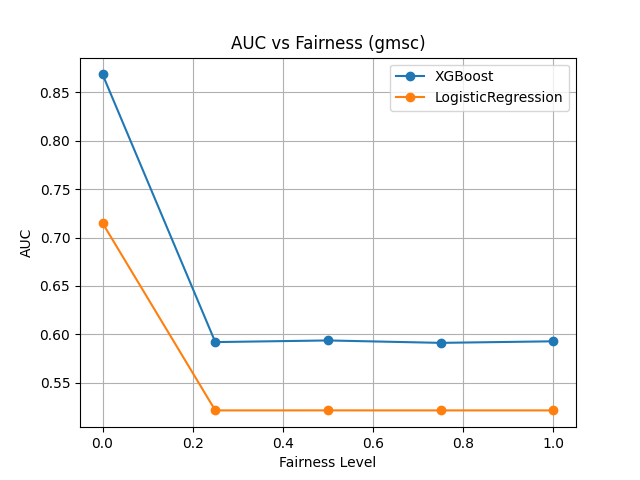
\includegraphics[width=0.8\textwidth]{images/gmsc_auc.png}
    \caption{AUC vs Fairness Level (GMSC)}
\end{figure}

\section{Statistical Testing}
\paragraph{}

To avoid relying only on one-time scores, I included statistical testing.

Cross-validation fold scores were aggregated using:
\begin{itemize}
    \item Mean
    \item Standard deviation
    \item 95\% confidence interval
\end{itemize}

Paired t-tests were used to compare baseline vs fairness-constrained performance at each fairness level. This helps check whether differences are likely real or just due to fold-level variation.

\begin{figure}[h!]
    \centering
    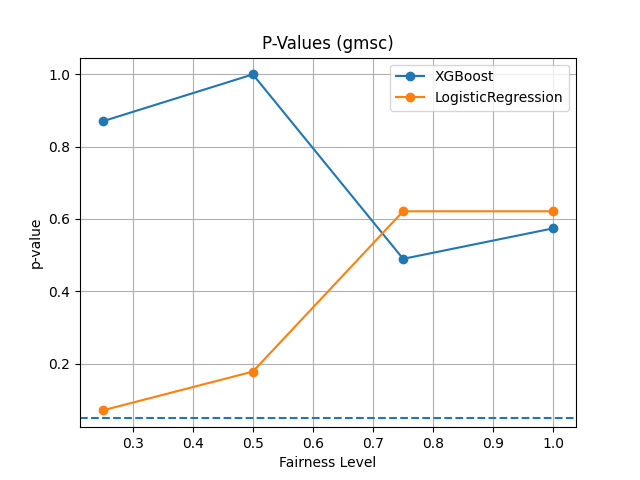
\includegraphics[width=0.8\textwidth]{images/gmsc_pvalues.png}
    \caption{Paired t-test p-values Across Fairness Levels (GMSC)}
\end{figure}

\begin{figure}[h!]
    \centering
    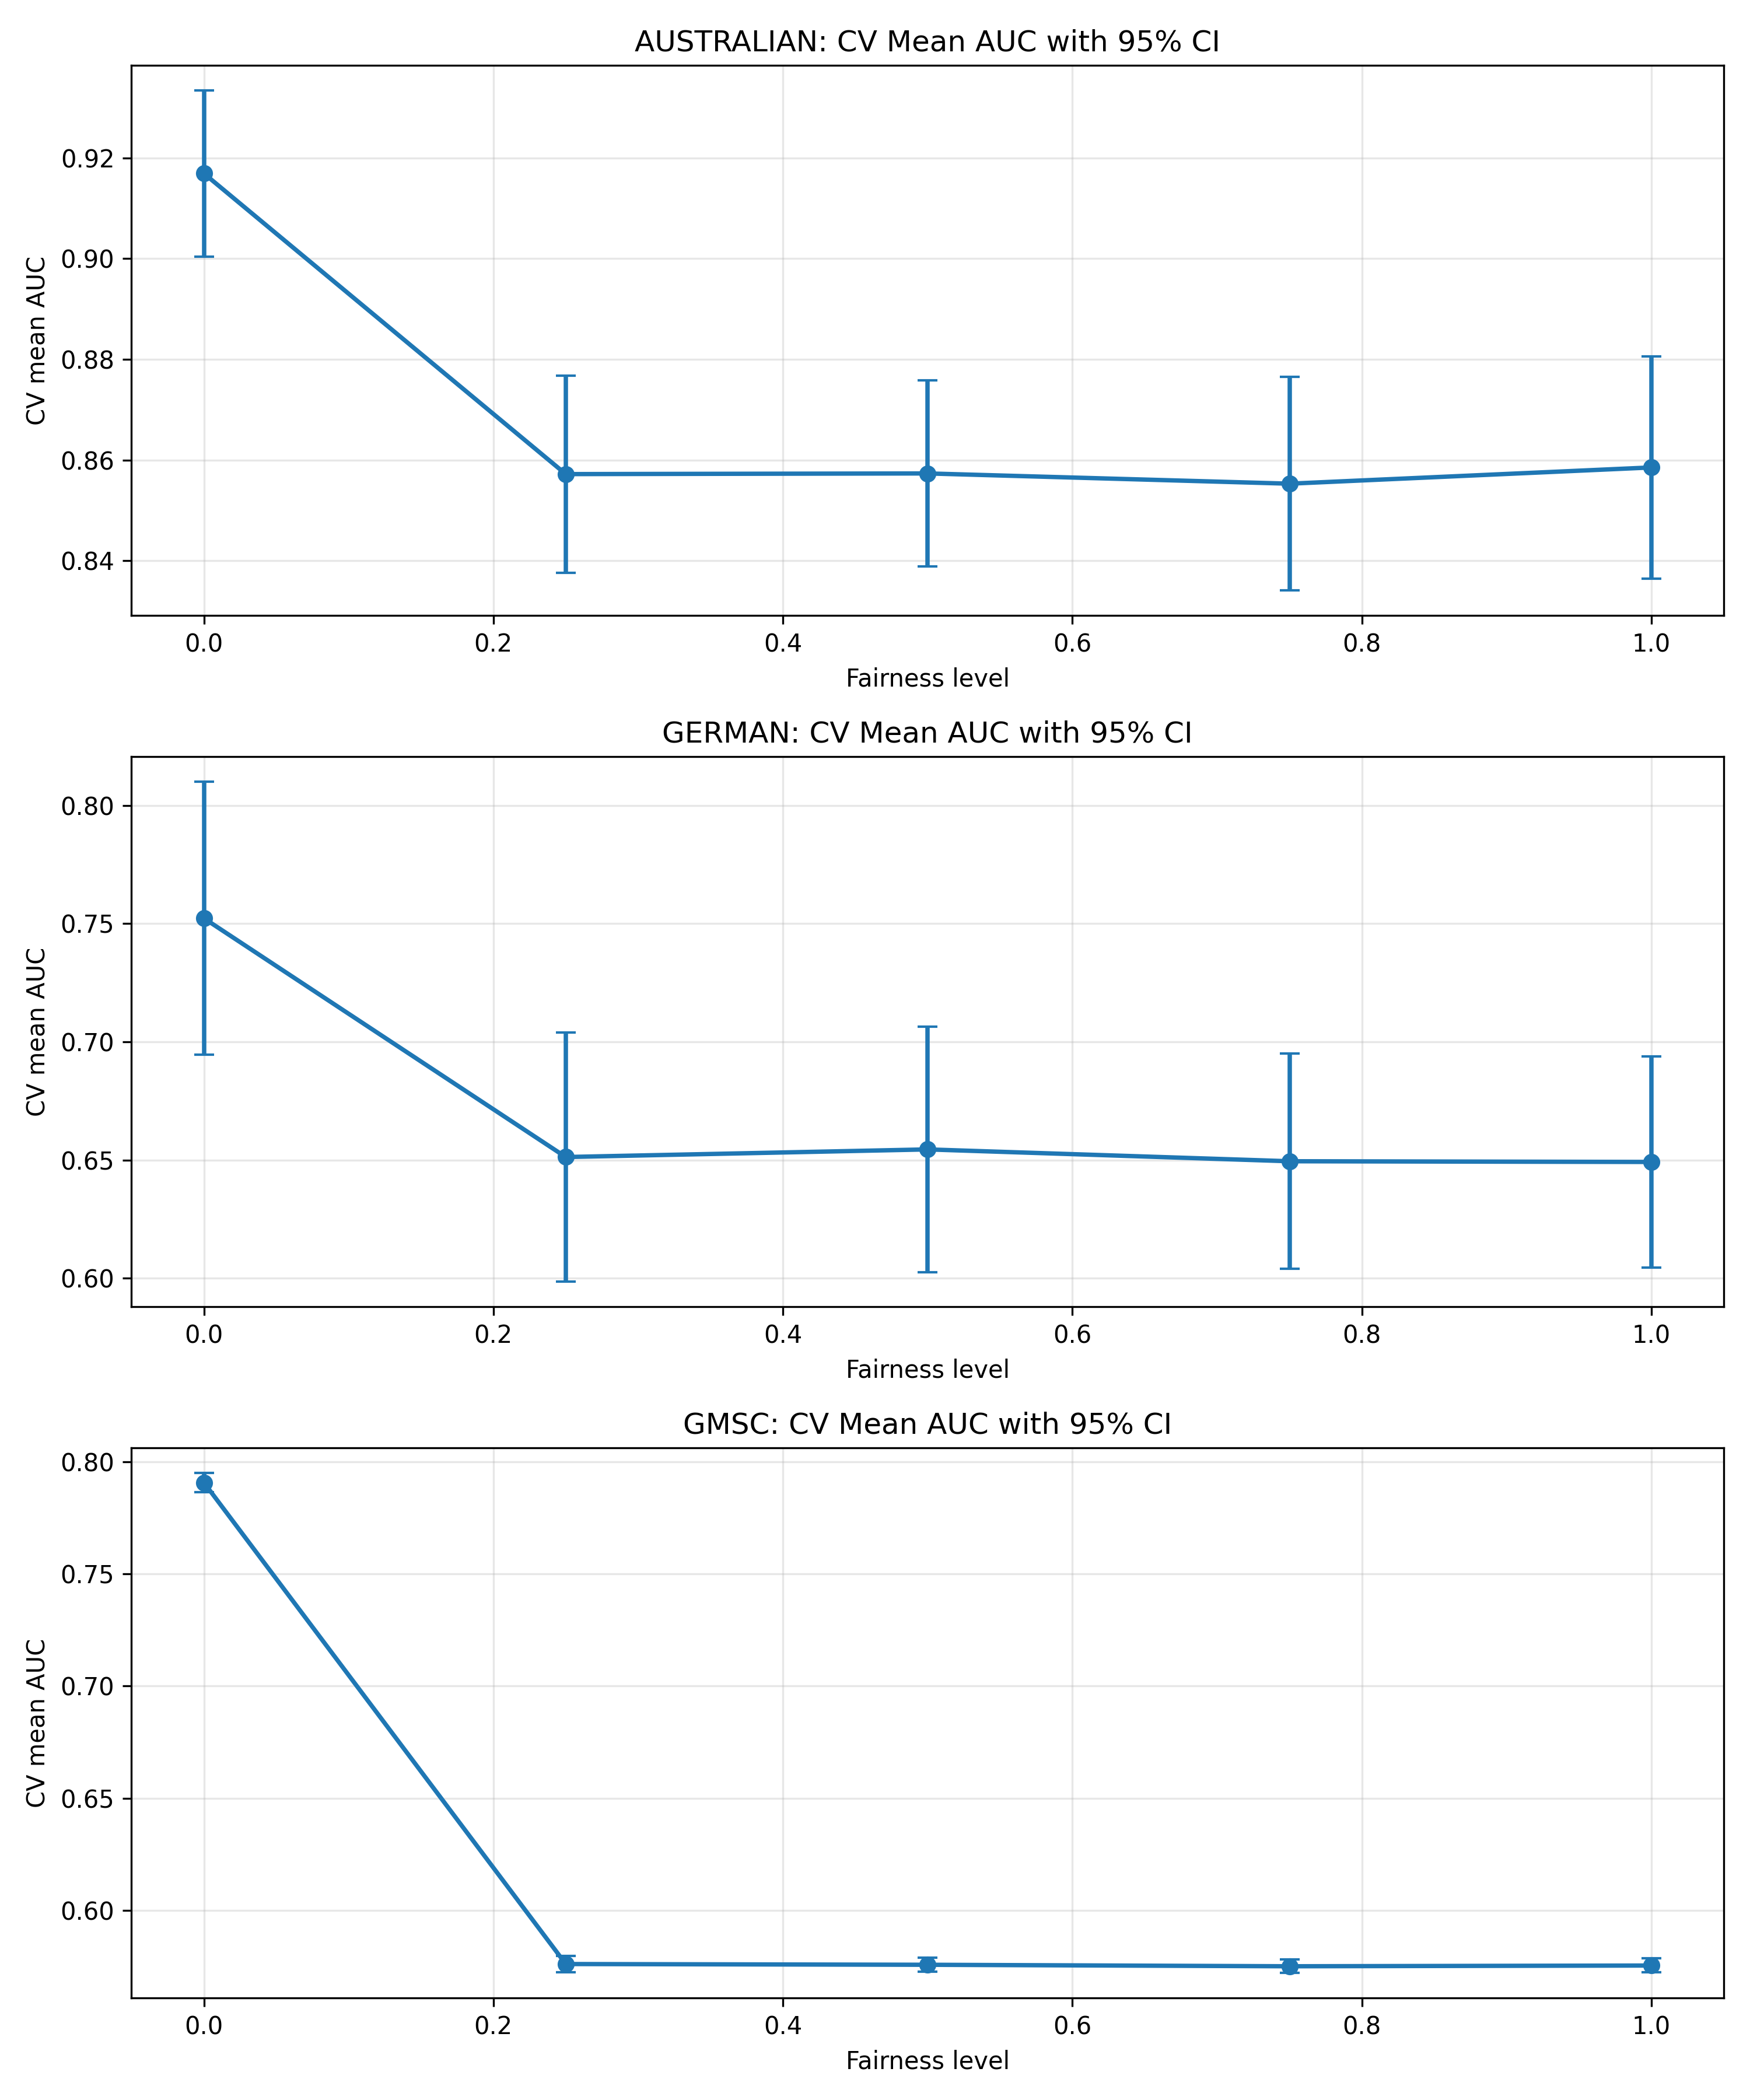
\includegraphics[width=0.8\textwidth]{images/figure_ci_auc_95.png}
    \caption{CV Mean AUC with 95\% Confidence Intervals (All Datasets)}
\end{figure}

\section{Testing Strategy}
\paragraph{}

The testing focus in this chapter is experimental validation (not unit testing of software functions).

I validated:
\begin{itemize}
    \item All model-fairness combinations are executed
    \item Outputs are generated in expected format
    \item Metric values stay in valid ranges
    \item Fold-based variability is reported through confidence intervals
\end{itemize}

\section{Reproducibility}
\paragraph{}

To make the work reproducible:
\begin{itemize}
    \item All experiment settings are controlled from config
    \item Random seed is fixed
    \item Preprocessing is consistent
    \item Outputs are saved in structured files
\end{itemize}

Main output files:
\begin{itemize}
    \item results.csv
    \item subgroup\_metrics.csv
    \item paired\_tests.csv
\end{itemize}

\begin{figure}[h!]
    \centering
    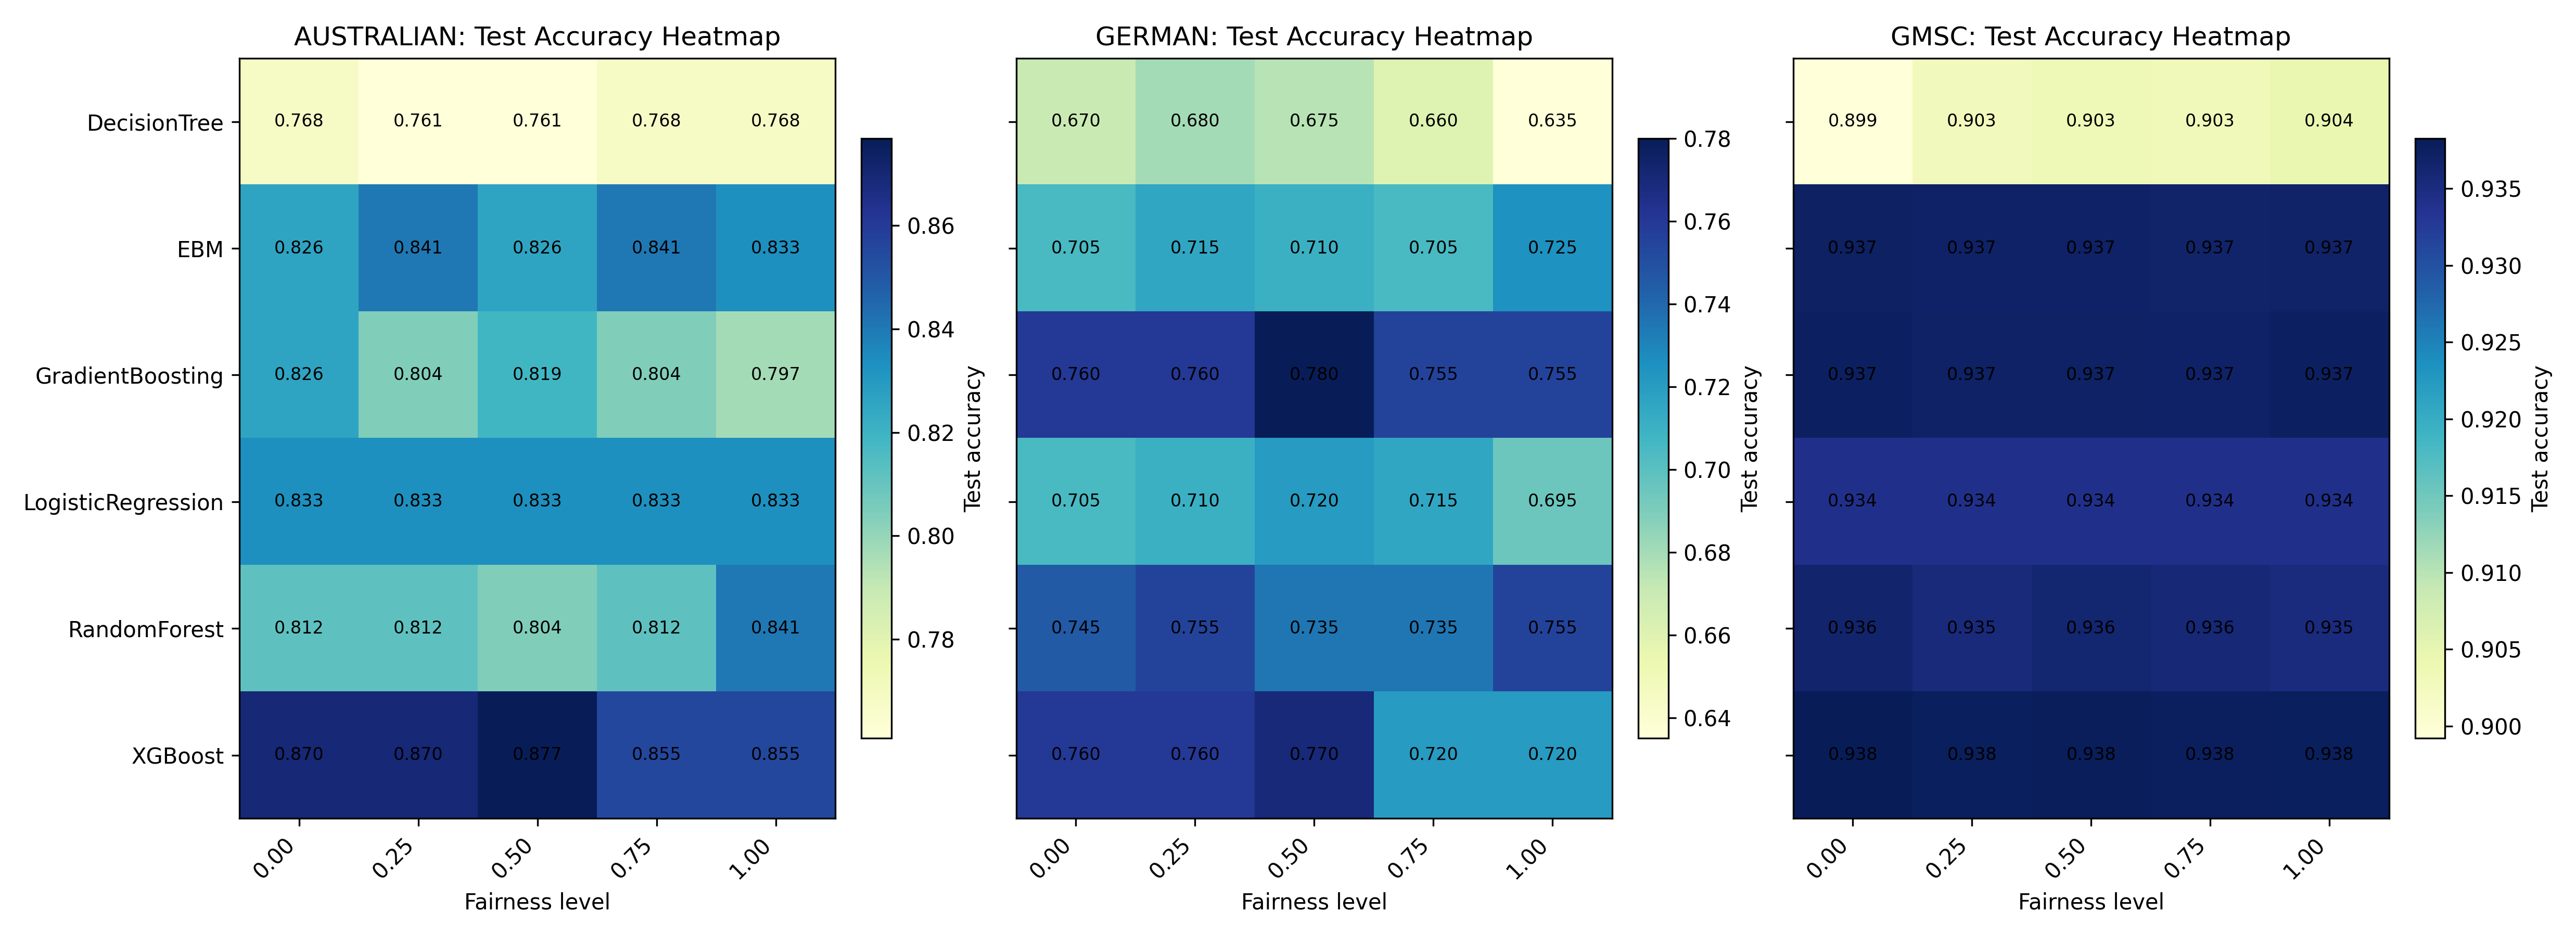
\includegraphics[width=0.85\textwidth]{images/figure_accuracy_heatmap.png}
    \caption{Test Accuracy Heatmap by Model and Fairness Level (All Datasets)}
\end{figure}

\section{Trade-off Validation Plot}
\paragraph{}

As a final methodology check, I used a direct fairness-performance trade-off plot to verify that fairness levels actually shift model behavior in expected ways.

\begin{figure}[h!]
    \centering
    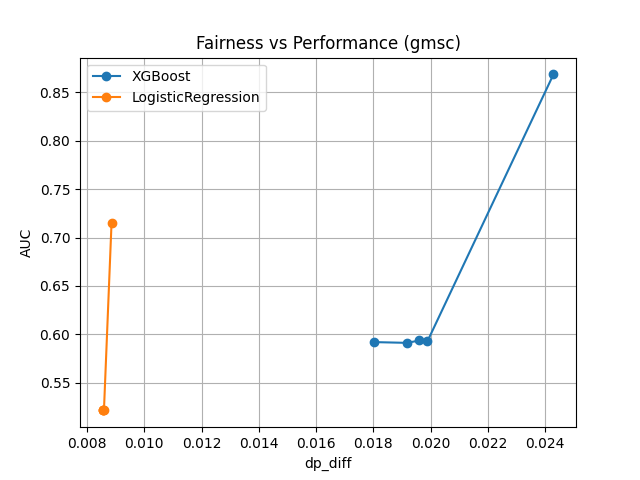
\includegraphics[width=0.85\textwidth]{images/gmsc_tradeoff.png}
    \caption{Fairness-Performance Trade-off Curve (GMSC)}
\end{figure}